\documentclass[12pt,a4paper]{article}
\usepackage{fontspec}
\defaultfontfeatures{Mapping=tex-text}
\usepackage{xunicode}
\usepackage[left=1cm,right=1.6cm,top=2cm,bottom=2cm]{geometry}
%\setmainfont{???}
\usepackage{amsmath}
\usepackage{amsfonts}
\usepackage{amssymb}
\usepackage{graphicx}
\author{Aquiles Carattino}
\title{Testing Image Resolution}
\begin{document}
\section*{72dpi}
\begin{center}
\includegraphics[width=3.54in]{72dpi.png}
\end{center}
This is text at 12pt
\section*{150dpi}
\begin{center}
\includegraphics[width=3.54in]{150dpi.png}
\end{center}
This is text at 12pt
\section*{300dpi}
\begin{center}
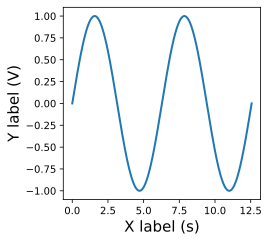
\includegraphics[width=3.54in]{300dpi.png}
\end{center}
\begin{center}
\includegraphics[width=7.25in, height=3.54in]{300dpi-full.png}
\end{center}
This is text at 12pt

\section*{600dpi}
\begin{center}
\includegraphics[width=3.54in]{600dpi.png}
\end{center}
\begin{center}
\includegraphics[width=7.25in]{600dpi-full.png}
\end{center}
This is text at 12pt

\end{document}

